\documentclass{report}
\usepackage[utf8]{inputenc}
\usepackage{graphicx}
\usepackage{subfigure}
\usepackage{subcaption}
\usepackage{biblatex}
\addbibresource{Citation.bib}
\usepackage{tabularx}
\usepackage{xcolor}
\usepackage[left= 1.8cm, right= 1.8cm, top=2cm, bottom=1.5cm]{geometry}
\usepackage{hyperref}
\usepackage{float}

\begin{document}

\begin{center}
    
\includegraphics[width=5cm]{Green_University_of_Bangladesh_logo.svg (1).png}
\end{center}
\vspace{0.4cm}
\begin{center}
    \LARGE \textbf{Green University of Bangladesh} \\
    \large \textbf{Department of Computer Science and Engineering} \\
    \textbf{Faculty of Sciences and Engineering}\\
    \textbf{Semester: (Spring, Year:2023), B.Sc. in CSE(Day)}\\
    \vspace{1.5cm}
   \large \textbf{Project Report}\\
    \large \textbf{Course Title: Integrated Design Project I Lab}\\
    \large \textbf{Course Code: CSE 324}\\
    \large \textbf{Section: PC 211 DA}\\
 \vspace{.8cm}
    \textbf{Project name:} Decentralized E-commerce Platform 
\vspace{1cm}

    \textbf{\underline{Student Details}}\\ 
     \vspace{0.5cm}

     \textbf{ \begin{tabular}{|>{\centering\arraybackslash}m{6cm}|>{\centering\arraybackslash}m{6cm}|}\hline
        Name & ID \\ \hline
       Md Emon Hossain  & 201902009 \\ \hline
        Md Kamrul Jaman Rabbi  & 211902012\\ \hline
    \end{tabular}}
   
    
\end{center}
\begin{center}
  \vspace{1.0cm}
\textbf{Submission Date: 13/06/2023}\\
\vspace{0.2 cm}
\textbf{Teacher's Name: Farjana Akter Jui}  
\end{center}
\vspace{1cm}
\textbf{\begin{center}
\begin{tabular}{|c c|}\hline
   \hspace{5cm}\underline{Project Report Status} &\\
    Marks: ............................... & Signature: ...............................\\
    Comments: ............................... & Date: ...............................\\ \hline
\end{tabular}
\end{center}}

\tableofcontents
\newpage
\chapter{Introduction}
\section{Introduction}
The rise of e-commerce has transformed the way people buy and sell goods and services. As
more people turn to online shopping, there is a growing need for e-commerce platforms that
are secure, efficient, and decentralized. In response to this need, a Decentralized E-commerce
Platform (DECP) has been developed to facilitate e-commerce transactions in a more secure
and efficient manner.
The DECP is designed to be a decentralized platform that eliminates the need for
intermediaries such as banks and payment processors. It is built on a blockchain technology
that allows for secure and transparent transactions between buyers and sellers. With the
DECP, buyers and sellers can conduct transactions without having to worry about the risk of
fraud, as the platform ensures that all transactions are transparent and verifiable.
This lab report will discuss the design and implementation of the DECP, including the features
and benefits of the platform. Additionally, it will provide an analysis of the platform’s
performance and potential use cases in the e-commerce industry

\section{Design Goals/Objective}
Here are the design goals and objectives of a decentralized e-commerce platform:

\subsection{Objectives}
\begin{itemize}
    \item Provide a secure and private e-commerce platform for users.
    \item Enable users to buy and sell goods and services without the need for a central authority.
    \item Reduce the cost of e-commerce transactions for businesses and consumers.
    \item Increase the speed and efficiency of e-commerce transactions.
    \item Improve the security and privacy of user data.
\end{itemize}
\subsection{Design Goals}
\begin{itemize}
    \item \textbf{Security:} The platform should be designed to be secure and resistant to cyberattacks.
    \item \textbf{Privacy:} The platform should respect user privacy and ensure that user data is not shared without their consent.
    \item \textbf{Scalability:} The platform should be designed to scale to meet the needs of a large number of users.
     \item \textbf{Efficiency:}The platform should be designed to be efficient and use resources wisely.
     \item \textbf{Interoperability:}The platform should be designed to be interoperable with other systems and platforms.
    
\end{itemize}
\newpage
\chapter{Design/Development/Implementation}

\section{Tools And Technologies}
Here are some of the tools and technologies that can be used to build a decentralized e-commerce platform:

\begin{itemize}
    \item \textbf{Blockchain:}Blockchain is a distributed ledger technology that can be used to store and track transactions. This makes it ideal for a decentralized e-commerce platform, as it provides a secure and tamper-proof way to store data.
    \begin{figure}[H]
        \centering
        
\includegraphics{tools/blockchain.jpeg}
        \caption{Blockchain}
        \label{fig:enter-label}
    \end{figure}

    \item \textbf{Decentralized storage: }Decentralized storage is a type of storage that is not controlled by a single entity. This makes it ideal for a decentralized e-commerce platform, as it provides a more secure and private way to store user data.
    \begin{figure}[H]
        \centering
        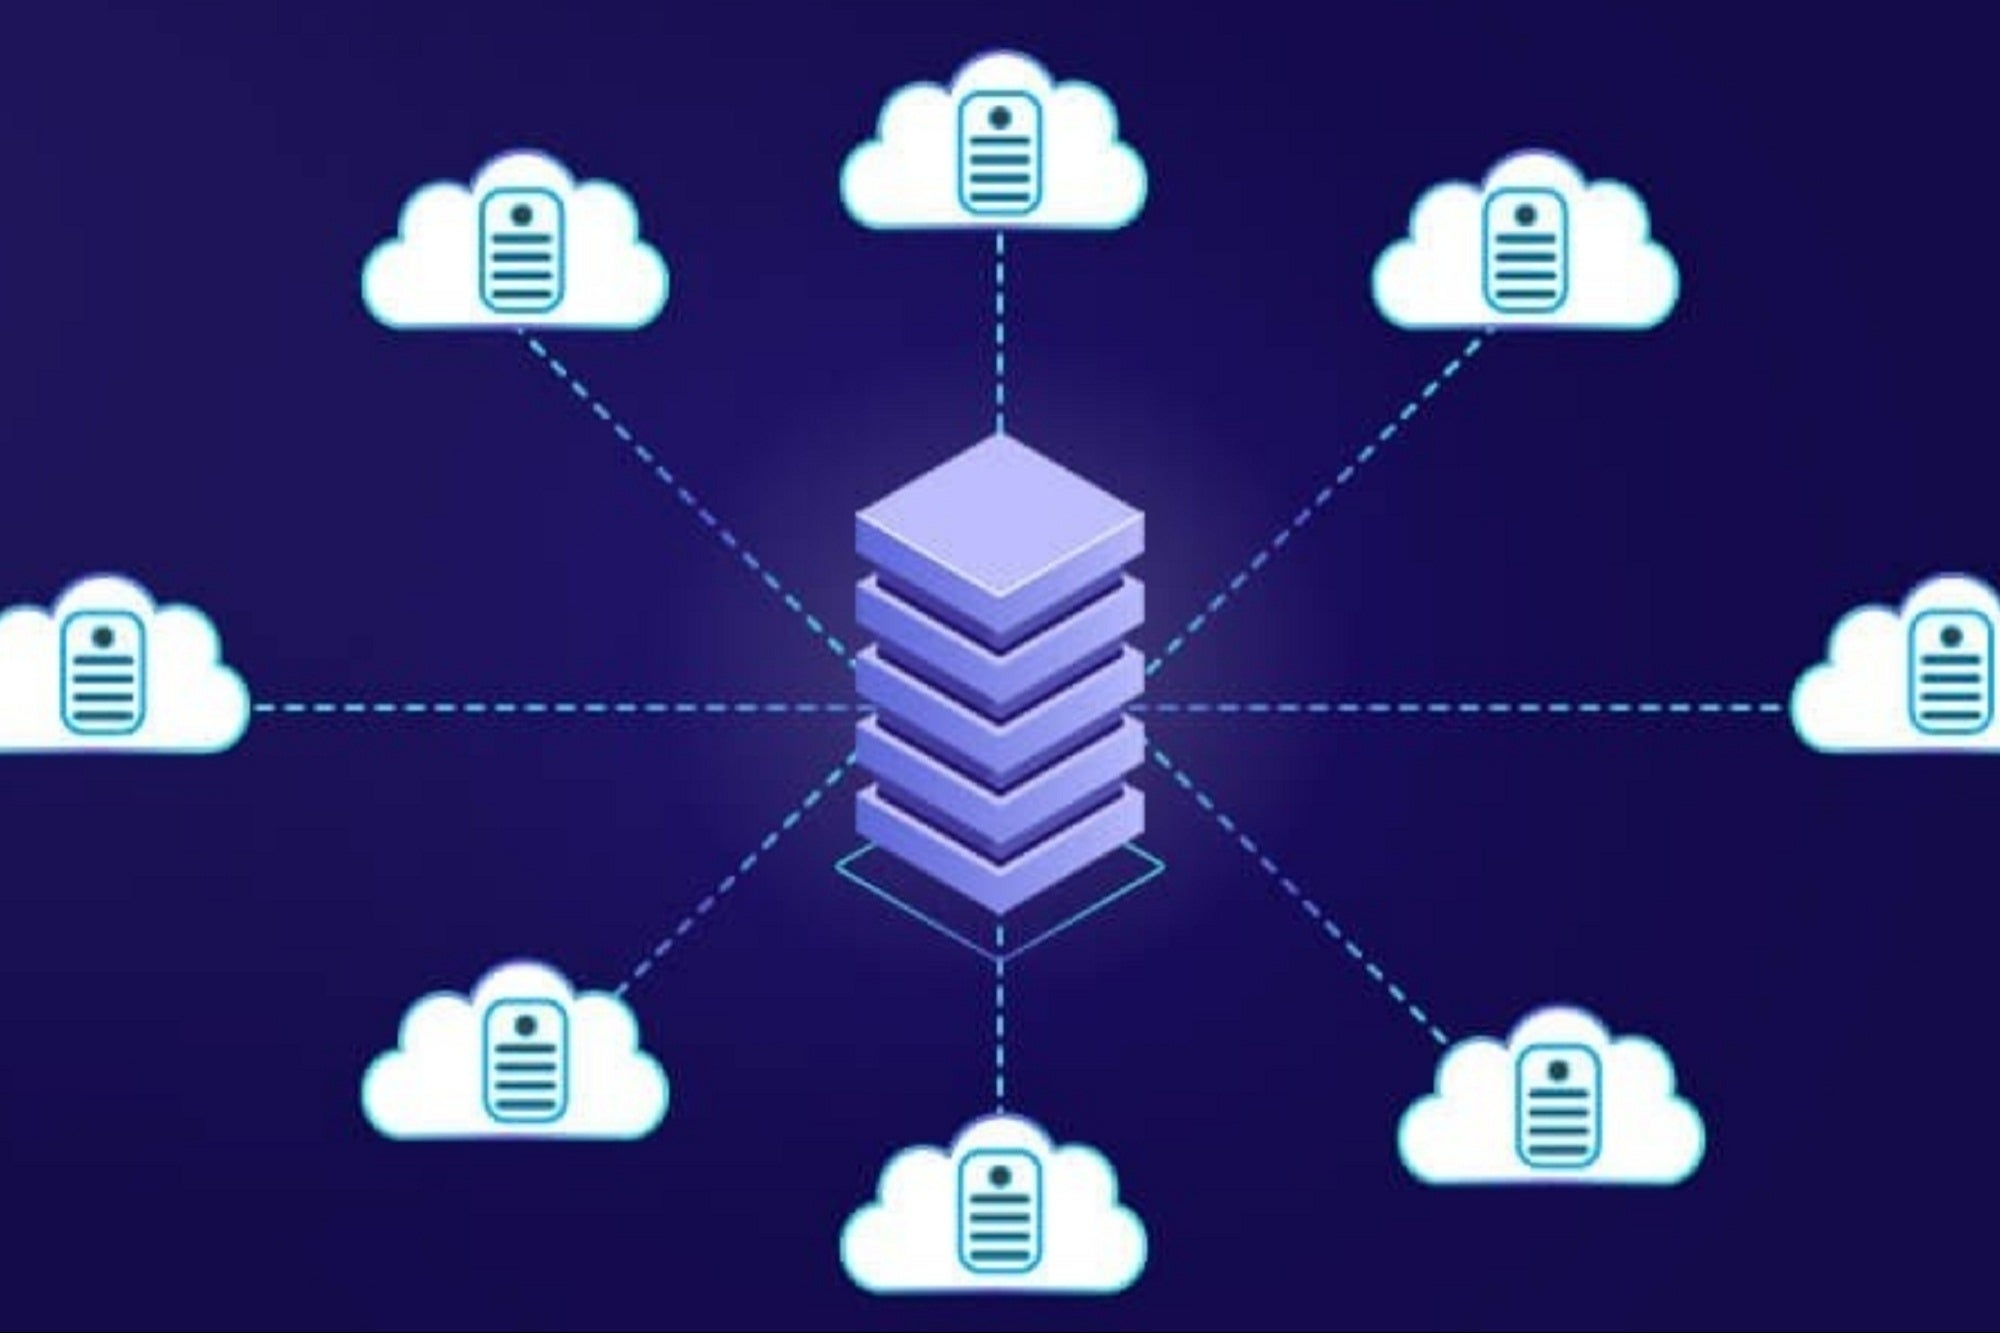
\includegraphics[width=8cm]{tools/decentralizestorge.jpg}
        \caption{Decentralized storage}
        \label{fig:enter-label}
    \end{figure}

    \item \textbf{Peer-to-Peer (P2P) Networks:}P2P networks enable direct communication and data sharing between buyers and sellers, bypassing the need for intermediaries. 
 \begin{figure}[H]
        \centering
        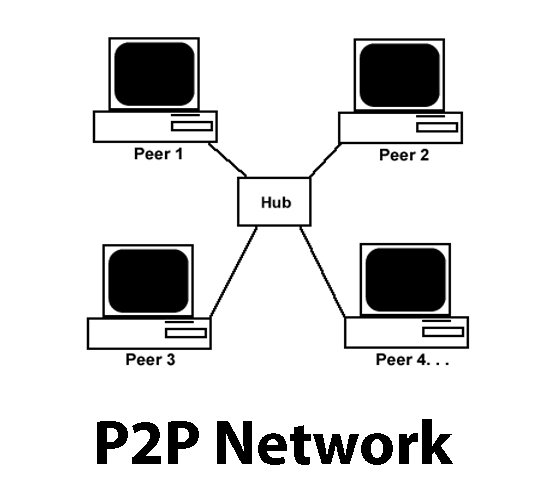
\includegraphics[width=8cm]{tools/peertopeer.jpg}
        \caption{Peer-to-Peer (P2P) Networks}
        \label{fig:enter-label}
    \end{figure}
    
\item \textbf{Smart Contracts:}Smart contracts are self-executing contracts with predefined rules encoded on the blockchain. They facilitate automated transactions and enforce trust between buyers and sellers. Solidity is a widely-used programming language for writing smart contracts on Ethereum.
 \begin{figure}[H]
        \centering
        
\includegraphics[width=8cm]{tools/smart-contract-featured-image-1.png}
        \caption{Smart Contracts}
        \label{fig:enter-label}
    \end{figure}

\end{itemize}

\section{Funtional Requirements}

  
  A decentralized e-commerce platform is a platform where buyers and sellers can connect without the need for intermediaries. Here are some functional requirements that such a platform should have:

\begin{enumerate}
        \item User Registration: The platform should allow users to register themselves as either buyers or sellers. \\
    
    \item User Profile: The platform should allow users to create and edit their profiles with details such as name, contact information, address, and payment details. \\

    \item  Product Catalog: The platform should have a catalog of products that are available for purchase. This catalog should be searchable and filterable.

\item Product Listing: Sellers should be able to create listings for their products. They should be able to add details such as product name, description, images, price, and shipping information
\item Product Management: Sellers should be able to manage their listings. They should be able to edit, delete, or mark their listings as sold.
\item Order Management: The platform should allow buyers to place orders for products. Sellers should be able to view and manage orders, mark orders as shipped, and communicate with buyers regarding the status of their orders.
\item Payment Gateway: The platform should integrate with a payment gateway to facilitate transactions between buyers and sellers.
\item Rating and Reviews: The platform should allow buyers to rate and review products and sellers. This feedback can help other buyers make informed decisions.
\item Messaging System: The platform should have a messaging system that allows buyers and sellers to communicate with each other.
\item Dispute Resolution: The platform should have a system in place to resolve disputes between buyers and sellers.
\item Security: The platform should have robust security measures in place to protect user data, prevent fraud, and ensure secure transactions.

\item Smart Contracts: The platform should use smart contracts to automate various processes such as payment and dispute resolution.
\item Interoperability: The platform should be interoperable with other decentralized e-commerce platforms to ensure a larger pool of buyers and sellers.
\item Decentralization: The platform should be truly decentralized, with no single entity controlling the platform or user data.
\end{enumerate}


\section{Non-functional Requirements} 


 In addition to functional requirements, non-functional requirements are also important for the success of a decentralized e-commerce platform.

\begin{enumerate}
    \item Performance: The platform should be able to handle a high volume of traffic and transactions without significant delays or downtime.
    \item Scalability: The platform should be able to scale up or down based on demand without compromising performance or functionality.
    \item Availability: The platform should be available 24/7 to users without any significant downtime or service interruptions.
    \item Reliability: The platform should be reliable and ensure that transactions are completed successfully and without errors.

    \item Security: The platform should be secure and protect user data and transactions from unauthorized access, fraud, and other security threats.
    \item Privacy: The platform should respect user privacy and ensure that user data is protected and not shared without explicit consent.
    \item Usability: The platform should be user-friendly and easy to navigate, with clear instructions and guidance for users.
    \item Accessibility: The platform should be accessible to users with disabilities and support assistive technologies.
    \item Sustainability: The platform should be environmentally sustainable and minimize its carbon footprint and energy consumption.
\end{enumerate}
\newpage
\section{Implementation}

 \textbf{Decentralized Network:} 
The first step in implementing a decentralized e-commerce platform is to establish a decentralized network. This can be achieved through the use of blockchain technology, which provides a distributed database that can be used to record and verify transactions. The decentralized network should be able to handle large volumes of transactions, ensure data privacy, and prevent double-spending.

\textbf{User Registration and Authentication:}
Once the decentralized network is established, the platform should allow users to register and authenticate themselves securely. The platform should use a decentralized identity system such as self-sovereign identity (SSI) to ensure the validity of user information. Users should be able to create accounts with their personal information and login credentials. The registration process should include email verification to ensure the validity of the user's email address.

\textbf{Product Management:}
The platform should allow vendors to upload their products for sale, including product descriptions, images, and pricing information. The product information should be stored on the decentralized network to ensure transparency and prevent tampering.

\textbf{Order Management:}
The platform should allow users to place orders for products, and vendors should be able to manage their orders. The platform should use smart contracts to automate the order management process, including payment processing and delivery tracking. The smart contracts should be stored on the decentralized network to ensure transparency and prevent tampering.\\


\textbf{Payment Processing:}
The platform should allow users to make payments using a variety of payment methods, including cryptocurrencies and traditional payment methods. The platform should use a decentralized payment system such as a blockchain-based payment system to ensure security and transparency.


\vspace{1cm}

\textbf{SDLC Models}

Selecting the right software development life cycle (SDLC) model is a crucial decision that can have a significant impact on the success of a software development project.

For a Decentralized E-commerce Platform, the Agile SDLC model is likely the most suitable choice. The Agile model is designed to be flexible and adaptive, which is particularly important for a decentralized platform, where requirements can change frequently. The Agile model is ideal for software development projects that require frequent iterations and updates, as well as continuous feedback from stakeholders.

\begin{figure}[H]
    \centering
    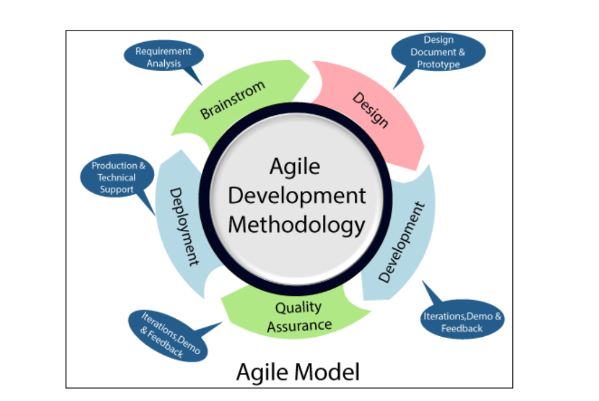
\includegraphics[width=8cm]{model/Screenshot from 2023-05-15 19-51-13.png}
    \caption{Agile Model}
    \label{fig:enter-label}
\end{figure}

In an Agile SDLC model, the development process is broken down into small iterations or sprints, where the team works on a specific set of tasks and delivers a working product at the end of each sprint. The Agile model allows for changes and updates to be made quickly and easily, which is particularly important for a Decentralized E-commerce Platform that requires constant updates to stay competitive in the marketplace.\\

\newpage
 \section{Data Flow Diagram}

A data flow diagram shows how data moves through an information system graphically. It may show the flow of stored data as well as incoming and outgoing data. The DFD makes no reference to how data moves around the system. It is a well-known visual illustration of how information moves through a system. A

clean and obvious DFD can graphically represent the appropriate quantity of the system need. It demonstrates how information enters and exits the system, what modifies the data, and where information is kept.
DFD and Flowchart differ significantly from one another. The flowchart shows how program modules' control flows. DFDs represent the different levels of data flow in the system. There are no branch or control elements in DFD.
 
 A decentralized e-commerce platform is a platform where buyers and sellers can connect without the need for intermediaries. A platform should have:

\begin{enumerate}
        \item User Registration: The platform should allow users to register themselves as either buyers or sellers. \\
    
    \item User Profile: The platform should allow users to create and edit their profiles with details such as name, contact information, address, and payment details. \\

    \item  Product Catalog: The platform should have a catalog of products that are available for purchase. This catalog should be searchable and filterable.

\item Product Listing: Sellers should be able to create listings for their products. They should be able to add details such as product name, description, images, price, and shipping information
\item Product Management: Sellers should be able to manage their listings. They should be able to edit, delete, or mark their listings as sold.
\item Order Management: The platform should allow buyers to place orders for products. Sellers should be able to view and manage orders, mark orders as shipped, and communicate with buyers regarding the status of their orders.
\item Payment Gateway: The platform should integrate with a payment gateway to facilitate transactions between buyers and sellers.
\item Rating and Reviews: The platform should allow buyers to rate and review products and sellers. This feedback can help other buyers make informed decisions.
\item Messaging System: The platform should have a messaging system that allows buyers and sellers to communicate with each other.
\item Dispute Resolution: The platform should have a system in place to resolve disputes between buyers and sellers.
\item Security: The platform should have robust security measures in place to protect user data, prevent fraud, and ensure secure transactions. 

\item Decentralization: The platform should be truly decentralized, with no single entity controlling the platform or user data.
\end{enumerate}

\newpage
\subsection{DFD Level-0,1,2 for decentralized ecomerce system}
\vspace{1cm}

In a Level-0 DFD (Data Flow Diagram), the focus is on providing an overview of the entire decentralized e-commerce system. It shows the major components of the system and their interactions at a high level, without going into detailed processes.
In the Level-1 DFD, the major processes in the system are decomposed into sub-processes:

User Registration and Authentication, Product Listing and Search, Payment Processing, Inventory Management, Review and Rating, User Account Management.

In the Level-2 Code DFD, each sub-function from the Level-1 DFD is further decomposed into more detailed functions or activities, following the same pattern.

\begin{enumerate}
    \item Performance: The platform should be able to handle a high volume of traffic and transactions without significant delays or downtime.
    \item Scalability: The platform should be able to scale up or down based on demand without compromising performance or functionality.
    \item Availability: The platform should be available 24/7 to users without any significant downtime or service interruptions.
    \item Reliability: The platform should be reliable and ensure that transactions are completed successfully and without errors.

    \item Security: The platform should be secure and protect user data and transactions from unauthorized access, fraud, and other security threats.
    \item Privacy: The platform should respect user privacy and ensure that user data is protected and not shared without explicit consent.
    \item Usability: The platform should be user-friendly and easy to navigate, with clear instructions and guidance for users.
    \item Accessibility: The platform should be accessible to users with disabilities and support assistive technologies.
    \item Sustainability: The platform should be environmentally sustainable and minimize its carbon footprint and energy consumption.
\end{enumerate}

\newpage
\begin{figure}[h]
    \centering
    
    \begin{minipage}{0.45\textwidth}
    \centering
    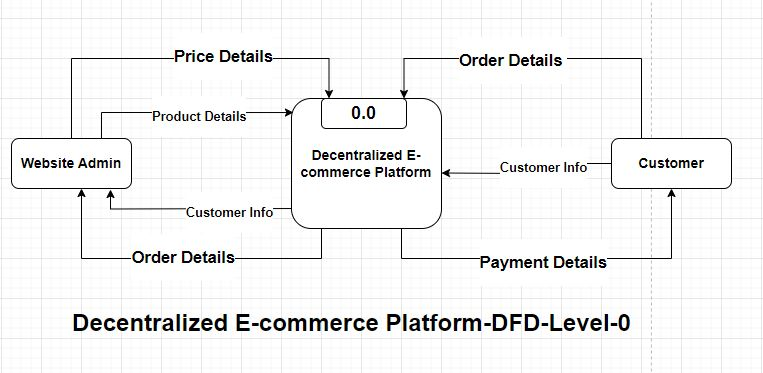
\includegraphics[width=1\textwidth]{dfd/dfd_level_0.jpeg}
    \caption{DFD level 0}
    \label{fig:1}
    \end{minipage}
    \hfill
    \begin{minipage}{0.45\textwidth}
    \centering
    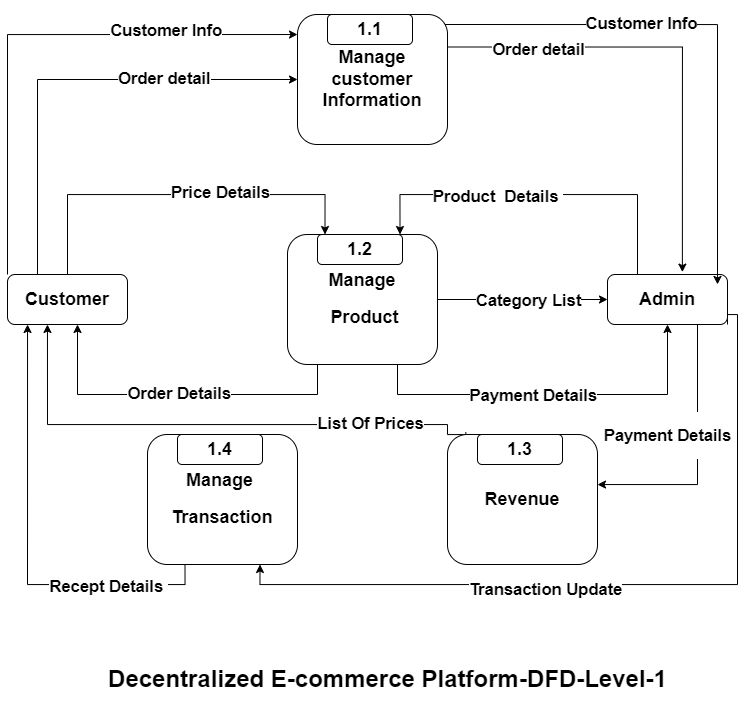
\includegraphics[width=1\textwidth]{dfd/dfd_level1.jpeg}
    \caption{DFD level 1}
    \label{fig:2}
    \end{minipage}  
\end{figure}

\begin{figure}[h]
    \centering
    
    \begin{minipage}{0.45\textwidth}
    \centering
    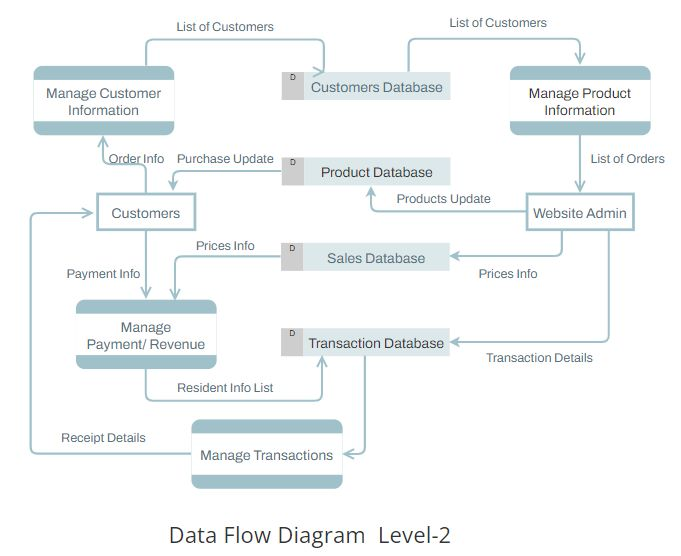
\includegraphics[width=1\textwidth]{dfd/dfd_level_2.jpeg}
    \caption{DFD level 3}
    \label{fig:3}
    \end{minipage}
    \hfill
    
    

\end{figure}

\newpage

\section{Use Case Diagram}
\begin{figure}[h]
    \centering
    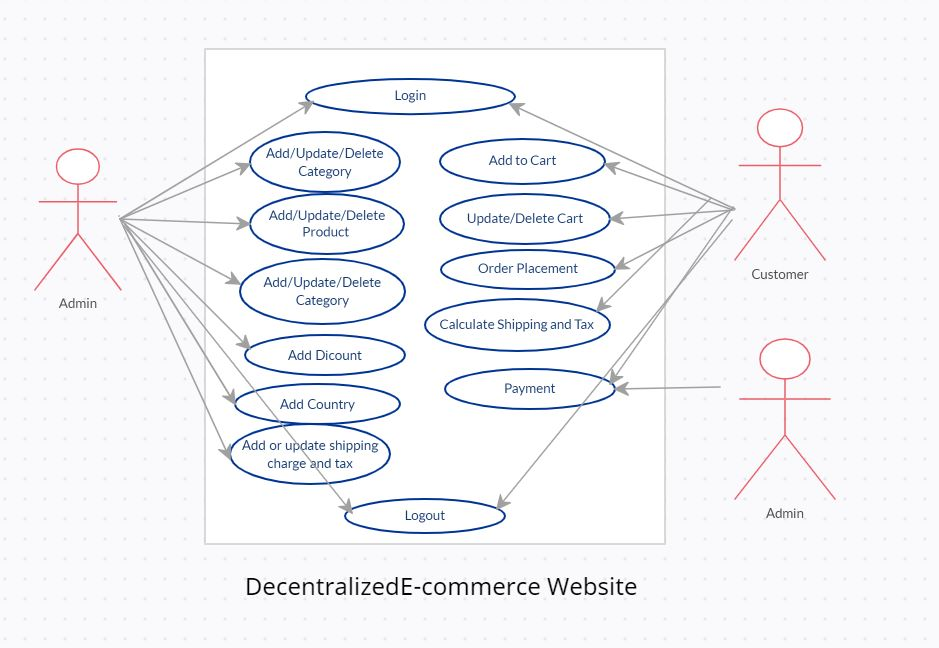
\includegraphics[width=10cm]{use_case_diagram/usecase_diagram.jpeg}
    \caption{use case diagram}
    \label{}
\end{figure}

Discovering the functional requirements from the problem statements of an intended system is challenging job.Use case represents the system’s functionality, the requirements of the system from the user’s perspective. A use case diagram is a dynamic or behavior diagram in UML.


\section{UML Class Diagram}

\begin{figure}[h]
    \centering
    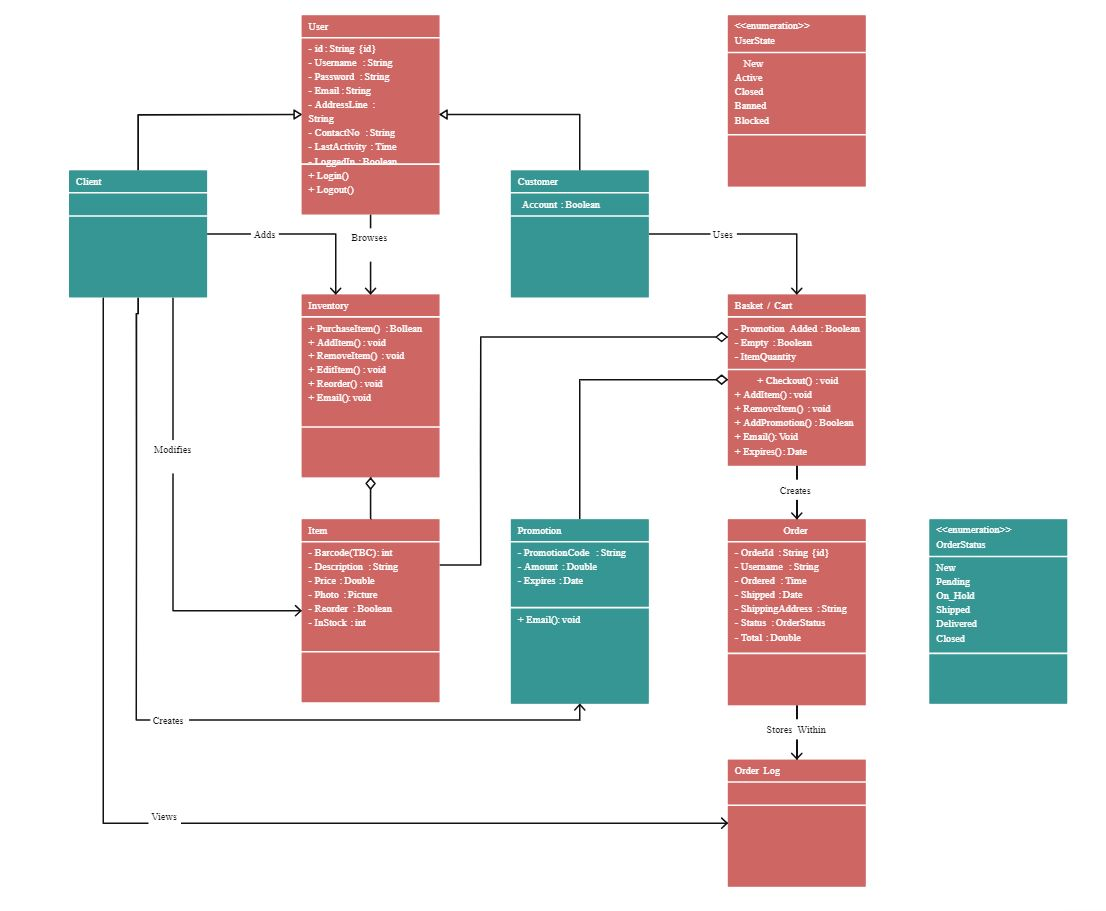
\includegraphics[width=10cm]{uml_class_diagram/uml_class_diagram.jpeg
    }
    \caption{UML Class Diagram}
    \label{}
\end{figure}


\chapter{Evaluation}


\begin{figure}[h]
    \centering
    
    \begin{minipage}{0.45\textwidth}
    \centering
    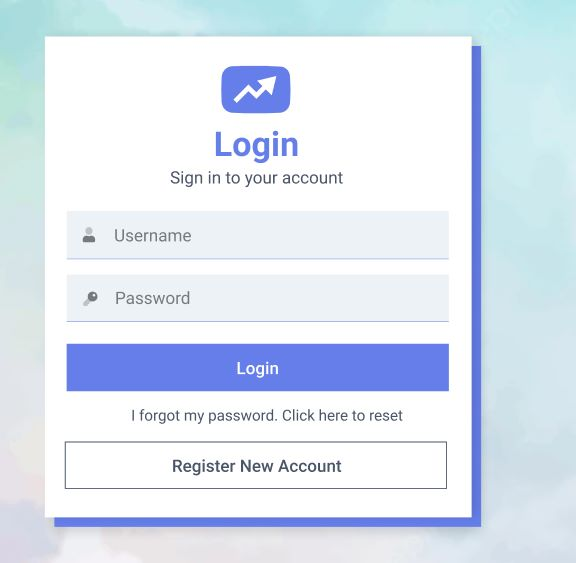
\includegraphics[width=7cm]{evaluation/01.jpeg}
    \caption{Login page}
    \label{fig:1}
    \end{minipage}
    \hfill
    \begin{minipage}{0.45\textwidth}
    \centering
    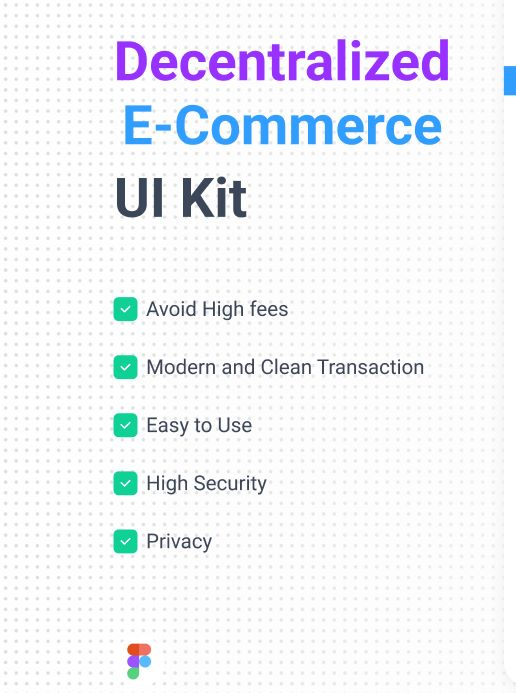
\includegraphics[width=7cm]{evaluation/02.jpeg}
    \caption{Features page}
    \label{fig:2}
    \end{minipage}  
\end{figure}

\begin{figure}[h]
    \centering
    
    \begin{minipage}{0.45\textwidth}
    \centering
    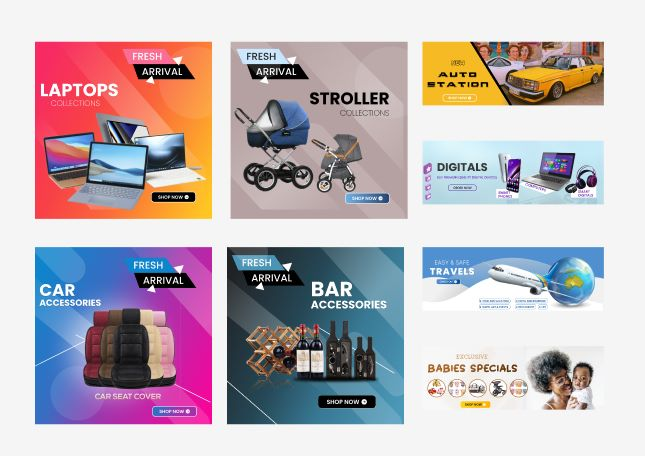
\includegraphics[width=7cm]{evaluation/03.jpeg}
    \caption{shopping page}
    \label{fig:3}
    \end{minipage}
    \hfill
    \begin{minipage}{0.45\textwidth}
    \centering
    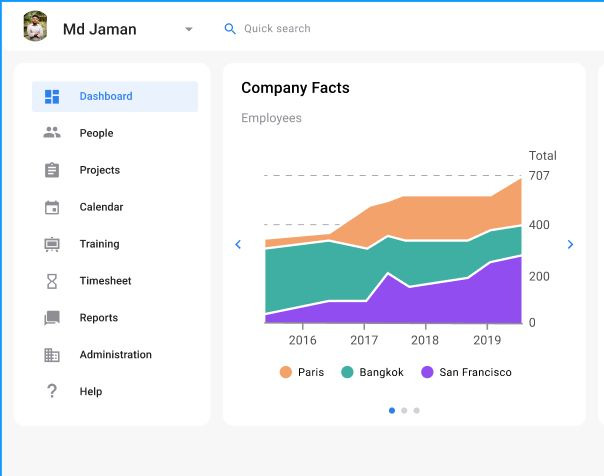
\includegraphics[width=7cm]{evaluation/04.jpeg}
    \caption{admin page}
    \label{fig:3}
    \end{minipage}
    

\end{figure}
\newpage

\chapter{Conclusion}

\section{Introduction}



Decentralized e-commerce platforms are a new and emerging way to buy and sell goods and services online. They offer a number of advantages over traditional e-commerce platforms, including:

\textbf{Security:} Decentralized platforms are more secure than traditional platforms because they do not store user data on a centralized server. This makes it much more difficult for hackers to steal data or commit fraud.

\textbf{Transparency:} Decentralized platforms are more transparent than traditional platforms because all transactions are recorded on a public blockchain. This allows users to see exactly how their data is being used and who is benefiting from their transactions.

\textbf{Efficiency:} Decentralized platforms are more efficient than traditional platforms because they do not require the use of third-party intermediaries. This can lead to lower fees and faster transaction times.

As the technology continues to develop, decentralized e-commerce platforms are likely to become more popular. They offer a number of advantages over traditional platforms, and they are well-positioned to disrupt the e-commerce market in the years to come.




\section{Practical Implications}

    


\textbf{Practical Implications of Decentralized E-commerce Platforms:}

\begin{itemize}
  \item \textbf{Increased security:} Decentralized e-commerce platforms do not store user data on a centralized server, which makes it much more difficult for hackers to steal data or commit fraud.
  \item \textbf{Reduced fees:} Decentralized e-commerce platforms do not require the use of third-party intermediaries, which can lead to lower fees for both buyers and sellers.
  \item \textbf{Improved transparency:} All transactions on a decentralized e-commerce platform are recorded on a public blockchain, which allows users to see exactly how their data is being used and who is benefiting from their transactions.
  \item \textbf{Increased control over data:} Users have complete control over their data on a decentralized e-commerce platform. They can choose to share their data with sellers or keep it private.
  \item \textbf{Increased trust:} Decentralized e-commerce platforms are built on trustless principles, which means that buyers and sellers do not need to trust each other in order to complete a transaction.
  \item \textbf{Increased flexibility:} Decentralized e-commerce platforms are not subject to the same regulations as traditional e-commerce platforms, which gives businesses more flexibility in how they operate.
  \item \textbf{Increased innovation:} Decentralized e-commerce platforms are still in their early stages, which means that there is a lot of room for innovation. Businesses can use decentralized e-commerce platforms to create new and innovative ways to buy and sell goods and services.
\end{itemize}

Overall, decentralized e-commerce platforms offer a number of practical benefits for both buyers and sellers. They are more secure, efficient, and transparent than traditional e-commerce platforms, and they offer users more control over their data and increased trust. As the technology continues to develop, decentralized e-commerce platforms are likely to become more popular and widespread.




\section{Scope of Future Work}

\begin{document}

\textbf{Scope and Future Works of Decentralized E-commerce Platform:}

\textbf{Scope:}

The scope of the decentralized e-commerce platform project includes the following key aspects:

\begin{itemize}
  \item Designing and implementing a decentralized architecture for the e-commerce platform.
  \item Integration of blockchain technology for secure and transparent transactions.
  \item Development of smart contracts to facilitate automated and trustless transactions between buyers and sellers.
  \item Implementation of decentralized identity solutions for enhanced privacy and security.
  \item Integration of peer-to-peer (P2P) networks for direct communication and data sharing between users.
  \item Building a user-friendly interface for seamless interaction with the platform.
\end{itemize}

\textbf{Future Works:}

There are several potential avenues for future work and enhancements in the field of decentralized e-commerce platforms:

\begin{itemize}
  \item \textbf{Scalability and Performance:} Future work can focus on improving the scalability and performance of the decentralized e-commerce platform to handle a larger number of transactions and users.
  \item \textbf{Integration with Real-World Applications:} Further development can involve integrating the decentralized e-commerce platform with real-world applications, such as supply chain management or decentralized finance (DeFi), to create a comprehensive ecosystem.
  \item \textbf{Enhanced User Experience:} Future work can concentrate on improving the user experience by implementing personalized recommendations, advanced search algorithms, and social features to enhance user engagement.
  \item \textbf{Cross-Chain Interoperability:} Research and development can explore cross-chain interoperability solutions to enable seamless communication and transactions between different blockchain networks.
  \item \textbf{Integration of AI and Machine Learning:} Leveraging AI and machine learning techniques can enhance fraud detection, product recommendations, and predictive analytics, providing more value to users.
  \item \textbf{Regulatory Compliance:} Future work can address regulatory challenges and ensure compliance with relevant laws and regulations to foster mainstream adoption of decentralized e-commerce platforms.
\end{itemize}

These future works aim to further advance decentralized e-commerce platforms, making them more efficient, user-friendly, and capable of addressing the evolving needs of users and businesses.


\documentclass{article}



\begin{thebibliography}{5}

\bibitem{kauffman2008}
Kauffman, B. (2008).
``Decentralism."
In R. Hamowy (Ed.),
\textit{The Encyclopedia of Libertarianism}.
Thousand Oaks, CA: Sage, Cato Institute.

\bibitem{deleon1994}
De Leon, D. (1994).
\textit{Leaders from the 1960s: A Biographical Sourcebook of American Activism}.
Greenwood Publishing Group.

\bibitem{roberts1984}
Roberts, N. L. (1984).
\textit{Dorothy Day and the Catholic worker}.
National security essay series, State University of New York Press.

\bibitem{walker2011}
Walker, J. (2011).
``Mark O. Hatfield, RIP."
\textit{Reason}, August 8.

\bibitem{loomis2005}
Loomis, M. J. (2005).
\textit{Decentralism: Where It Came From – Where Is It Going?}.
Black Rose Books.

\end{thebibliography}



\end{document}
  




